\chapter{Macdonald polynomials} \label{chap:polynomials}

% \todo[inline]{Add chapter introduction explaining the overall structure and goals.}

% Throughout this chapter, let \(n\) be a nonnegative integer.

\section{Permutations and compositions}

The \vocab{symmetric group} \(\sym{n}\) is
the group of all permutations of the set
\(\interval{n} = \{1, 2, \ldots, n\}\).
We write permutations in one-line notation
\(\sigma = \window{\sigma_1, \sigma_2, \ldots, \sigma_n}\).
Given two permutations \(\sigma, \pi \in \sym{n}\),
their product is the permutation \(\sigma \pi \in \sym{n}\)
defined by \((\sigma \pi)_i = \sigma_{\pi_i}\).
The \vocab{reverse} \(\rev(\sigma)\) of
a permutation \(\sigma \in \sym{n}\) is the permutation
\(\rev(\sigma) = \sigma w_0 = \window{\sigma_n, \sigma_{n-1}, \dots, \sigma_1}\),
where \(w_0 = \window{n, n-1, \cdots, 1}\).
The symmetric group \(\sym{n}\) is generated by
the \vocab{simple transpositions} \(s_1, s_2, \ldots, s_{n-1}\),
where \(s_i \in \sym{n}\) is the permutation that swaps the elements \(i\) and \(i+1\) and fixes all other elements.
The \vocab{length} \(\ell(\sigma)\) of a permutation \(\sigma \in \sym{n}\) is
the smallest number of simple transpositions whose product equals \(\sigma\).
A \vocab{reduced expression} of a permutation \(\sigma\) is
a sequence \(s_{i_1},s_{i_2},\ldots,s_{i_{\ell(\sigma)}}\) of simple transpositions
whose product \(s_{i_1}s_{i_2}\cdots s_{i_{\ell(\sigma)}}\) equals \(\sigma\).

A \vocab{composition of length \(n\)} is a sequence
\(\alpha = \composition{\alpha_1, \alpha_2, \ldots, \alpha_n}\)
of nonnegative integers.
A \vocab{partition} is a weakly decreasing composition,
and an \vocab{antipartition} is a weakly increasing composition.
Given a composition \(\alpha\), let \(\dec(\alpha)\) and \(\inc(\alpha)\) denote
the partition and antipartition obtained by sorting the parts of \(\alpha\)
in weakly decreasing and weakly increasing order, respectively.
Define \(\rev(\alpha)=\composition{\alpha_n, \alpha_{n-1}, \ldots, \alpha_1}\)
to be the composition given by reversing the parts of \(\alpha\).

The \vocab{exponent notation} for a composition \(\alpha = \composition{\alpha_1, \ldots, \alpha_n}\)
is given by a sequence of nonnegative integers \(p_1, p_2, \ldots, p_k\)
and positive integers \(m_1, m_2, \ldots, m_k\) that sum to \(n\)
such that \(p_i \neq p_{i+1}\) for \(i\in[k-1]\), written as
\begin{equation*}
	\alpha = \composition{
		\underbrace{p_1 p_1 \ldots p_1}_{m_1},
		\underbrace{p_2 p_2 \ldots p_2}_{m_2},
		\ldots,
		\underbrace{p_k p_k \ldots p_k}_{m_k}
	} = p_1^{m_1} p_2^{m_2} \ldots p_k^{m_k}.
\end{equation*}

The \vocab{conjugate} of a partition \(\lambda\) is the partition \(\lambda'\) defined by
\begin{equation*}
	\lambda'_i = |\{ j \suchthat \lambda_j \geq i \}|.
\end{equation*}

Given a permutation \(\pi \in \sym{n}\) and a composition \(\alpha = \composition{\alpha_1, \ldots, \alpha_n}\),
the \vocab{left action} of \(\pi\) on \(\alpha\) is the composition
\(\pi \permact \alpha = \composition{\alpha_{\pi^{-1}(1)}, \alpha_{\pi^{-1}(2)}, \ldots, \alpha_{\pi^{-1}(n)}}\).
In particular,
this choice of notation guarantees that
\(\sigma \permact (\pi \permact \alpha) = (\sigma \pi) \permact \alpha\)
for all \(\sigma, \pi \in \sym{n}\) and
\(\alpha=\composition{\alpha_1,\ldots,\alpha_n}\).
Note that \(\rev(\alpha) = w_0 \permact \alpha\).

\begin{example}
	For example, \(\alpha=\composition{3, 1, 0, 2, 2, 0}\) is
	a composition of length \(6\) with exponent notation \(3^11^10^12^20^1\).
	It rearranges to the partition \(\dec(\alpha) = \composition{3, 2, 2, 1, 0, 0}\),
	the antipartition \(\inc(\alpha) = \composition{0, 0, 1, 2, 2, 3}\),
	and \(\rev(\alpha)=\composition{0,2,1,0,2,3}\).
	The permutation \(\pi = \window{3, 1, 2, 4, 6, 5}\) has reduced expression \(s_2s_1s_5\).
	The result of the left action of \(\pi\) on \(\alpha\) is
	the composition \(\pi \permact \alpha = \composition{1, 0, 3, 2, 0, 2}\),
	with a graphical representation shown in \Cref{fig:left-action-on-composition}.
\end{example}

\begin{figure}[htbp]
	\centering
	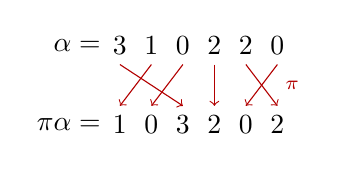
\begin{tikzpicture}[x=.4cm, y=-.5cm]
		\node[anchor=east] at (0.7, 0) {\(\alpha = \)};
		\foreach \i [count = \j] in {3, 1, 0, 2, 2, 0}{
				\node (A\j) at (\j, 0) {\(\i\)};
			}
		\node[anchor=east] at (0.7, 2) {\(\pi \permact \alpha = \)};
		\foreach \i [count = \j] in {1, 0, 3, 2, 0, 2}{
				\node (B\j) at (\j, 2) {\(\i\)};
			}
		\node[anchor=east, color=red!70!black] at (7, 1) {\(\scriptstyle \pi\)};
		\foreach \i [count = \j] in {3, 1, 2, 4, 6, 5}{
				\draw[->, color=red!70!black] (A\j.south) -- (B\i.north);
			}
	\end{tikzpicture}
	\caption{
		The left action of \(\pi = \window{3, 1, 2, 4, 6, 5}\)
		on \(\alpha = \composition{3, 1, 0, 2, 2, 0}\).
	}
	\label{fig:left-action-on-composition}
\end{figure}

\begin{remark}
	Given permutations \(\sigma, \pi \in \sym{n}\) and
	a composition \(\alpha=\composition{\alpha_1,\ldots,\alpha_n}\),
	\cite{Ale19} writes \(\pi \alpha\) to mean \(\pi \permact \alpha\),
	and writes \(\pi \sigma\) to mean \(\pi \permact \sigma\),
	interpreting \(\sigma\) as a composition,
	which we write as a product \(\pi \sigma^{-1}\).
\end{remark}

\section{Symmetric functions and plethystic notation}

We assume basic familiarity with the ring \(\Lambda(F)\) of symmetric functions in countably infinitely many variables \(\mathbf{x} = (x_1, x_2, \ldots)\) with coefficients in a field \(F\) of characteristic zero.
This includes important families of symmetric functions,
such as the power sum symmetric functions \(p_k\),
and the Schur functions \(s_\lambda\).
We refer the reader to \cite[Chapter~7]{EC2} for a comprehensive introduction to this topic.
We take the coefficient field to be \(F = \rationals(q, t)\), the field of rational functions in the variables \(q\) and \(t\) with rational coefficients.

Recall that the \vocab{power sum symmetric functions} \(p_k\) for \(k \geq 1\) are defined by
\begin{equation*}
	p_k = \sum_{i \geq 1} x_i^k.
\end{equation*}
Any symmetric function can be uniquely expressed as a polynomial in the power sum symmetric functions.
In other words,
\begin{equation*}
	\Lambda(F) = F[p_1, p_2, p_3, \ldots].
\end{equation*}
We adopt plethystic notation as in \cite[Section~2]{Hai99}, defined as follows.

Let \(A\) be a formal series (not necessarily symmetric, and not necessarily with \(x_1, x_2, \dots\) as indeterminates).
We define \(p_k[A]\) to be the formal series obtained by replacing each indeterminate \(a\) in \(A\) by \(a^k\) (including the indeterminates \(q\) and \(t\), if they appear in \(A\)).
For a symmetric function \(f \in \Lambda(F)\), let
\begin{equation*}
	f = Q_f(p_1, p_2, \ldots, p_m)
\end{equation*}
be the expression of \(f\) as a polynomial \(Q_f\) in the power sum symmetric functions.
Then, the \vocab{plethystic substitution} of \(A\) into \(f\) is defined as
\begin{equation*}
	f[A] = Q_f(p_1[A], p_2[A], \ldots, p_m[A]).
\end{equation*}

If \(A\) is a sum of indeterminates, \(A = a_1 + a_2 + \cdots\), then \(p_k[A] = a_1^k + a_2^k + \cdots = p_k(a_1, a_2, \ldots)\), and thus \(f[A] = f(a_1, a_2, \ldots)\).
This explains why we call \(f[A]\) a kind of substitution.
Similarly, if \(A\) is a sum of monomials, then \(f[A]\) is \(f\) evaluated on these monomials.
An important example is
\[
	f[1/(1-t)] = f[1 + t + t^2 + t^3 + \cdots] = f(1, t, t^2, t^3, \ldots).
\]

We let \(X = x_1 + x_2 + x_3 + \cdots\) denote the sum of all indeterminates in \(\mathbf{x}\).
Then, \(f[X] = f(\mathbf{x})\) is the usual evaluation of \(f\) at the variables \(\mathbf{x}\), and
\[
	f[X/(1-t)] = f(x_1, x_2, x_3, \ldots, t x_1, t x_2, t x_3, \ldots, t^2 x_1, t^2 x_2, t^2 x_3, \ldots ).
\]
Note that some manipulations are easier in plethystic notation;
for example, if \(g(\mathbf{x})  = f[X/(1-t)]\), then \(f(\mathbf{x}) = g[X(1-t)]\).

\section{Algebraic definitions of Macdonald polynomials}

In this section, we define multiple variations of Macdonald polynomials:
\begin{itemize}
	\item \(P_\mu\), the symmetric Macdonald polynomials,
	\item \(J_\mu\), the integral form symmetric Macdonald polynomials,
	\item \(\tilde{H}_\mu\), the modified Macdonald polynomials,
	\item \(E_\alpha^\sigma\), the permuted-basement (nonsymmetric) Macdonald polynomials,
	\item \(\mathcal{E}_\alpha^\sigma\), the integral form permuted-basement (nonsymmetric) Macdonald polynomials.
\end{itemize}

\subsection{Symmetric Macdonald polynomials \texorpdfstring{\(P_\mu\)}{Pμ}}

We follow \cite[Chapter VI]{Mac96} for the definition of symmetric Macdonald polynomials.

Define the scalar product \(\langle \cdot, \cdot \rangle_{(q, t)}\) on \(\Lambda(\rationals(q, t))\) by
\begin{equation*}
	\langle p_\lambda, p_\mu \rangle_{(q, t)} = \delta_{\lambda\mu} z_\lambda \prod_{i=1}^{\ell(\lambda)} \frac{1 - q^{\lambda_i}}{1 - t^{\lambda_i}},
\end{equation*}
where \( z_\lambda = \prod_{i \geq 1} i^{m_i} m_i!\), with \(m_i\) being the multiplicity of the part \(i\) in the partition \(\lambda\).
When \(q = t\), this scalar product reduces to the usual Hall inner product on symmetric functions.
% If \(q, t\) are treated as real parameters lying in \( (0, 1) \), then the scalar product is positive definite.

\begin{theorem}[{\cite[Theorem~4.7]{Mac96}}]
	There exists a unique family of symmetric functions (called \vocab{symmetric Macdonald polynomials}) \(P_\lambda = P_\lambda(\mathbf{x}; q, t) \in \Lambda(\rationals(q, t))\) indexed by partitions \(\lambda\) such that
	\begin{itemize}
		\item \( P_\lambda = m_\lambda + \sum_{\mu < \lambda} u_{\lambda\mu}(q, t) m_\mu \) with coefficients \( u_{\lambda\mu}(q, t) \in \rationals(q, t) \), and;
		\item \( \langle P_\lambda, P_\mu \rangle_{(q, t)} = 0 \quad \text{if } \lambda \ne \mu \).
	\end{itemize}
\end{theorem}

For any polynomial \( f(x_1, \ldots, x_n) \) and \(1 \le i \le n\), define the \(q\)-shift operator \(T_{q,x_i}\) by
\begin{equation*}
	(T_{q,x_i} f)(x_1, \ldots, x_n) = f(x_1, \ldots, qx_i, \ldots, x_n).
\end{equation*}
Then, the operator \( D \) is defined as
\begin{equation*}
	D = \sum_{i=1}^n \left( \prod_{j \ne i} \frac{t x_i - x_j}{x_i - x_j} \right) T_{q,x_i}.
\end{equation*}
The operator \(D\) has distinct eigenfunction, and these eigenfunctions are the symmetric Macdonald polynomials \(P_\lambda(x_1, \ldots, x_n; q, t)\) where \(\lambda\) is a partition with at most \(n\) parts.

\subsection{Integral form symmetric Macdonald polynomials \texorpdfstring{\(J_\mu\)}{Jμ}}

We define the integral form symmetric Macdonald polynomials following \cite[Chapter VII, Section 8]{Mac04}.

For a partition \(\mu\), define the \vocab{normalization factor \(c_\mu(q, t)\)} by
\begin{equation} \label{eq:normalization-factor-c-mu}
	c_\mu(q, t) = \prod_{u \in \dg(\mu)} (1 - q^{\leg(u)} t^{\arm(u)+1}),
\end{equation}
where the product is over all boxes \(u\) in the skyline diagram \(\dg(\mu)\) of \(\mu\), and \(\leg(u)\) and \(\arm(u)\) are the leg and arm lengths of the box \(u\) in \(\dg(\mu)\), respectively.
The notions of skyline diagrams, leg lengths, and arm lengths are defined in \Cref{subsec:non-augmented-fillings}.%
\footnote{
	The exponents of \(q\) and \(t\) in the formula in \cite[Chapter VII, Section 8]{Mac04} are \(a(u)\) and \(l(u)+1\), where \(a(u)\) and \(l(u)\) denote the arm and leg lengths of the box \(u\) in the Young diagram of \(\mu\).
	Our formula measures arm and leg lengths in the skyline diagram, which effectively swaps the roles of arms and legs compared to the Young diagram.
	Hence the apparent swap of arms and legs is due to the different diagram conventions, and our formula is consistent with that in \cite{Mac04}.
}
For now, it suffices to note \(c_\mu(q,t)\) is a polynomial in \(q\) and \(t\) that admits an explicit formula.

The \vocab{integral form symmetric Macdonald polynomial} \(J_\mu = J_\mu(\mathbf{x}; q, t)\) is defined by
\begin{equation} \label{eq:J-algebraic-definition}
	J_\mu(\mathbf{x}; q, t) = c_\mu(q, t) P_\mu(\mathbf{x}; q, t).
\end{equation}
The naming ``integral form'' is due to the fact that
the coefficients of \(J_\mu(\mathbf{x}; q, t)\)
are polynomials in \(q\) and \(t\) with integer coefficients.
Several proofs of this integrality result appeared in the late 1990s; for example, \cite{Kno97}.

\subsection{Modified Macdonald polynomials \texorpdfstring{\(\tilde{H}_\mu\)}{H̃μ}}

We define the modified Macdonald polynomials following \cite[Section~2]{Hai99}.
The \vocab{modified Macdonald polynomial} \(\tilde{H}_\mu = \tilde{H}_\mu(\mathbf{x}; q, t)\) is defined by the plethystic substitution
\begin{equation} \label{eq:modified-macdonald-plethystic}
	\tilde{H}_\mu(\mathbf{x}; q, t) = t^{n(\mu)} J_\mu\left[ \frac{X}{1 - t^{-1}}; q, t^{-1} \right],
\end{equation}
where \(n(\mu) = \sum_{i \geq 1} (i-1) \mu_i\).

\begin{proposition}[{\cite[Proposition~2.6]{Hai99}}] \label{prop:modified-macdonald-characterization}
The modified Macdonald polynomials \(\tilde{H}_\mu\) satisfy and are uniquely determined by the following properties:
\(\tilde{H}_\mu[X(1 - q); q, t]\) is a linear combination of Schur functions \(s_\lambda\) with \(\lambda \geq \mu\) in dominance order;
\(\tilde{H}_\mu[X(1 - t); q, t]\) is a linear combination of Schur functions \(s_\lambda\) with \(\lambda \geq \mu'\) in dominance order; and
\(\langle \tilde{H}_\mu, s_{(n)} \rangle = 1\).
\end{proposition}

\subsection{Permuted-basement Macdonald polynomials \texorpdfstring{\(E_\alpha^\sigma\)}{Eασ}}
\label{sec:permuted basement def}

We follow the exposition of \cite{Fer11} and the notation of \cite{Ale19}
for the definition of nonsymmetric Macdonald polynomials
and permuted-basement Macdonald polynomials,
which are polynomials in the ring \(\rationals(q, t)[\mathbf{x}_n] = \rationals(q, t)[x_1, x_2, \ldots, x_n]\).
For more background on this topic, see \cite{GR22},
where these polynomials are referred to as the \emph{relative Macdonald polynomials}.

Recall that a permutation \(\sigma \in \sym{n}\) acts on
a polynomial \(f(\mathbf{x})\) by permuting the variables,
that is,
\(\sigma (\mathbf{x}^{\alpha}) = \mathbf{x}^{\sigma \permact \alpha}\)
for a composition \(\alpha\).
For example, the permtutation \(\sigma = \window{2, 3, 1}\) sends the monomial \(x_1^2 x_2 = \mathbf{x}^{\composition{2, 1, 0}}\) to the monomial
\(
	\window{2, 3, 1} (x_1^2 x_2)
	= \window{2, 3, 1}(\mathbf{x}^{\composition{2, 1, 0}})
	= \mathbf{x}^{\window{2, 3, 1} \permact \composition{2, 1, 0}}
	= \mathbf{x}^{\composition{0, 2, 1}}
	= x_2^2 x_3
\).

The \vocab{Demazure--Lusztig operators}
\(T_1\), \dots, \(T_{n-1}\) on \(\rationals(q, t)[\mathbf{x}]\)
are defined by
\begin{equation*}
	T_i(f) = ts_i(f) + (1-t) x_{i+1} \frac{f - s_i(f)}{x_i - x_{i+1}},
\end{equation*}
for \(i \in \interval{n-1}\),
and the operator \(g\) on \(\rationals(q, t)[\mathbf{x}]\) is defined by
\begin{equation*}
	g(f(x_1, \ldots, x_n)) = f(x_2, x_3, \ldots, x_n, q^{-1}x_1).
\end{equation*}
For a reduced expression \( \sigma = s_{i_1} \cdots s_{i_k} \),
we write \(T_\sigma\) to denote the composition \(T_{i_1} \circ \cdots \circ T_{i_k}\).
The \vocab{Cherednik--Dunkl operators}
\(Y_1\), \dots, \(Y_n\) on \(\rationals(q, t)[\mathbf{x}]\)
are defined by,
for each \(i \in \interval{n}\),
\begin{equation*}
	Y_i = t^{i-1} T_{i-1}^{-1} \cdots T_1^{-1} g T_{n-1} \cdots T_i.
\end{equation*}

\begin{definition}[{\cite[Theorem 4.1.4]{Fer11}}]
	For a composition \(\alpha=\composition{\alpha_1,\ldots,\alpha_n}\),
	the \vocab{nonsymmetric Macdonald polynomial} \(E_\alpha=E_\alpha(\mathbf{x}; q, t)\) is
	the unique element of \(\rationals(q, t)[\mathbf{x}]\) such that
	the coefficient of \(\mathbf{x}^{\alpha}\) is \(1\),
	and for all \(i\in\interval{n}\),
	\begin{equation*}
		Y_i E_\alpha = q^{-\alpha_i} t^{k_i} E_\alpha,
	\end{equation*}
	where
	\(
	k_i = |\{ j \in \interval{i-1} \suchthat \alpha_j > \alpha_i \}|
	+ |\{ j \in \interval{i+1, n} \suchthat \alpha_j \geq \alpha_i \}|
	\).
\end{definition}

\begin{remark}
	We note that there is a typo in \cite{Fer11}:
	the corresponding formula for \(k_i\) has a minus sign instead of a plus sign.
	Our formulation aligns with the definition in \cite{Kno97},
	although the notation there differs.
\end{remark}

\begin{example}
	\label{example:nonsymmetric-macdonald-polynomial}
	Let \(n = 4\) and \(\alpha = \composition{1, 0, 1, 1}\).
	Then, \(k_1 = 2\), \(k_2 = 3\), \(k_3 = 1\) and \(k_4 = 0\).
	Therefore, the nonsymmetric Macdonald polynomial
	\(E_{\composition{1, 0, 1, 1}}(\mathbf{x}; q, t)\)
	is the unique element of \(\rationals(q, t)[x_1, x_2, x_3, x_4]\) such that
	the coefficient of \(x_1 x_3 x_4\) is \(1\), and
	\begin{align*}
		Y_1 E_{\composition{1, 0, 1, 1}} & = q^{-1} t^{2} E_{\composition{1, 0, 1, 1}}, &
		Y_2 E_{\composition{1, 0, 1, 1}} & = q^{0}  t^{3} E_{\composition{1, 0, 1, 1}},   \\
		Y_3 E_{\composition{1, 0, 1, 1}} & = q^{-1} t^{1} E_{\composition{1, 0, 1, 1}}, &
		Y_4 E_{\composition{1, 0, 1, 1}} & = q^{-1} t^{0} E_{\composition{1, 0, 1, 1}}.
	\end{align*}
	The unique polynomial satisfying the above is
	\begin{equation*}
		E_{\composition{1, 0, 1, 1}}(x_1, x_2, x_3, x_4; q, t)
		=
		x_1 x_2 x_3 \frac{1 - t}{1 - q t^2} +
		x_1 x_2 x_4 \frac{1 - t}{1 - q t^2} +
		x_1 x_3 x_4.
	\end{equation*}
\end{example}

The following definition is a reformulation based on \cite[Corollary 16]{Ale19} and \cite[Remark 4.4.5]{Fer11}.

\begin{definition}[Permuted-basement Macdonald polynomials]
	\label{definition:permutedbasement}
	For a composition \(\alpha=\composition{\alpha_1,\ldots,\alpha_n}\)
	and a permutation \(\sigma \in \sym{n}\),
	the \vocab{permuted-basement Macdonald polynomial}
	\(E_\alpha^\sigma = E_{\alpha}^{\sigma}(\mathbf{x}; q, t)\)
	is given by
	\begin{equation*}
		E_{\alpha}^{\sigma} =
		t^{-\twinv(\alpha, \sigma)} T_{\rev(\sigma)} E_{\rev(\alpha)},
	\end{equation*}
	where
	\(
	\twinv(\alpha, \sigma) =
	\left| \{
	(i, j) \suchthat
	i < j \text{ and }
	\alpha_i \geq \alpha_j \text{ and }
	\sigma_i < \sigma_j
	\} \right|
	\).
\end{definition}

Note that, for \(\sigma = w_0 = \window{n, n-1, \ldots, 1}\),
the permuted-basement Macdonald polynomial \(E_{\alpha}^{w_0}(\mathbf{x}; q, t)\)
is the nonsymmetric Macdonald polynomial \(E_{\rev(\alpha)}(\mathbf{x}; q, t)\).

\begin{remark}
	\label{remark:notation-permuted-basement-macdonald-polynomial-Ale19}
	Our notation for the permuted-basement Macdonald polynomial agrees with
	the notation in \cite{Ale19,CMW22},
	which is different from the notation in \cite{Fer11}.
	Notably, the permuted-basement Macdonald polynomial \(E_{\alpha}^{\sigma}(\mathbf{x}; q, t)\)
	is denoted by \(E_{\rev(\alpha)}^{\rev(\sigma)}(\mathbf{x};q,t)\) in \cite{Fer11}.
\end{remark}

\begin{remark}
	We note a typo in \cite{Ale19} concerning the definition of \(\twinv(\alpha, \sigma)\):
	the inequality involving \(\sigma\) is reversed.
	This error becomes apparent by considering the special case \(E_\alpha^{w_0}\).
	Our formulation aligns with the definition provided in \cite{Fer11},
	although we use different notation.
\end{remark}

\begin{example}
	\label{example:permuted-basement-macdonald-polynomial}
	Let \(n = 4\),
	\(\alpha = \composition{1, 1, 0, 1}\),
	and \(\sigma = \window{2, 4, 1, 3}\).
	Then, \(\rev(\sigma)=\window{3, 1, 4, 2}\) has reduced expression \(s_2 s_1 s_3\),
	so the Demazure--Lusztig operator \(T_{\rev(\sigma)}\) is given by \(T_2 T_1 T_3\).
	We compute
	\(
	\twinv(\alpha, \sigma) =
	\twinv(\composition{1, 1, 0, 1}, \window{2, 4, 1, 3}) =
	|\{(1, 2), (1, 4)\}| = 2
	\).
	Therefore,
	the permuted-basement Macdonald polynomial
	\(E_{\composition{1, 1, 0, 1}}^{\window{2, 4, 1, 3}}(\mathbf{x}; q, t)\)
	is given by
	\begin{equation*}
		E_{\composition{1, 1, 0, 1}}^{\window{2, 4, 1, 3}}(\mathbf{x}; q, t)
		=
		t^{-2}
		T_2 T_1 T_3
		E_{\composition{1, 0, 1, 1}}(\mathbf{x}; q, t),
	\end{equation*}
	which can be computed from \cref{example:nonsymmetric-macdonald-polynomial} as
	\begin{equation*}
		E_{\composition{1, 1, 0, 1}}^{\window{2, 4, 1, 3}}
		=
		x_{1} x_{2} x_{3} \frac{t(1 - t)}{1 - q t^2} +
		x_{1} x_{3} x_{4} \frac{1 - t}{1 - q t^2} +
		x_{2} x_{3} x_{4}.
	\end{equation*}
\end{example}

\begin{example}
	\label{example:permuted-basement-macdonald-polynomial-2}
	Let \(n = 4\),
	\(\alpha = \composition{1, 1, 0, 1}\),
	and \(\tau = \window{4, 2, 1, 3}\).
	Then, \(\rev(\tau) = \window{3, 1, 4, 2}\) has a reduced expression \(\rev(\tau) = s_2 s_1\),
	so the Demazure--Lusztig operator \(T_{\rev(\tau)}\) is given by \(T_2 T_1\).
	We compute
	\(
	\twinv(\alpha, \tau) =
	\twinv(\composition{1, 1, 0, 1}, \window{4, 2, 1, 3}) =
	|\{(1, 4)\}| = 1
	\).
	Therefore, the permuted-basement Macdonald polynomial
	\(E_{\composition{1, 1, 0, 1}}^{\window{4, 2, 1, 3}}(\mathbf{x}; q, t)\)
	is given by
	\begin{equation*}
		E_{\composition{1, 1, 0, 1}}^{\window{4, 2, 1, 3}}(\mathbf{x}; q, t)
		=
		t^{-1}
		T_2 T_1
		E_{\composition{1, 0, 1, 1}}(\mathbf{x}; q, t),
	\end{equation*}
	which can be computed as
	\begin{equation*}
		E_{\composition{1, 1, 0, 1}}^{\window{4, 2, 1, 3}}
		=
		x_{1} x_{2} x_{3} \frac{t(1 - t)}{1 - q t^2} +
		x_{1} x_{3} x_{4} \frac{1 - t}{1 - q t^2} +
		x_{2} x_{3} x_{4}.
	\end{equation*}
\end{example}

Note that the computations in \Cref{example:permuted-basement-macdonald-polynomial} and \Cref{example:permuted-basement-macdonald-polynomial-2} yield the same result, which exemplifies a property that will be explored in \Cref{chap:probabilistic}.

\begin{theorem}[{\cite{Fer11}}]
	Let \(\sigma\) be a permutation in \(\sym{n}\).
	The set of permuted-basement Macdonald polynomials
	\begin{equation*}
		\{ E_\alpha^\sigma(\mathbf{x}; q, t) \suchthat
		\alpha \text{ is a composition of length } n \}
	\end{equation*}
	is a basis of \(\rationals(q, t)[\mathbf{x}]\).
\end{theorem}

\subsection{Integral form permuted-basement Macdonald polynomials \texorpdfstring{\(\mathcal{E}_\alpha^\sigma\)}{Eασ}}

We define the integral form permuted-basement Macdonald polynomials following \cite[Section~5]{Kno97}.
While \cite{Kno97} only defined the integral form nonsymmetric Macdonald polynomials (i.e., the case \(\sigma = w_0\)),
the extension to the permuted-basement case is straightforward by using the same normalization factor.

For a composition \(\alpha=\composition{\alpha_1,\ldots,\alpha_n}\), define the \vocab{normalization factor \(d_\alpha(q, t)\)} by
\begin{equation} \label{eq:normalization-factor-d-alpha}
	d_\alpha(q, t) = \prod_{u \in \dg(\alpha)} (1 - q^{\leg(u)+1} t^{\arm(u)+1}),
\end{equation}
where the product is over all boxes \(u\) in the skyline diagram \(\dg(\alpha)\) of \(\alpha\), and \(\leg(u)\) and \(\arm(u)\) are the leg and arm lengths of the box \(u\) in \(\dg(\alpha)\), respectively.
The notions of skyline diagrams, leg lengths, and arm lengths are defined in \Cref{subsec:non-augmented-fillings}.%
\footnote{
	The exponents of \(q\) and \(t\) in the formula in \cite[Section~5]{Kno97} are \(a(u)+1\) and \(l(u)+1\).
	We call \(\leg(u)\) the quantity that \cite{Kno97} denotes by \(a(u)\), and \(\arm(u)\) the quantity that \cite{Kno97} denotes by \(l(u)\).
	Hence our formula is consistent with that in \cite{Kno97}.
}
The \vocab{integral form permuted-basement Macdonald polynomial} \(\mathcal{E}_\alpha^\sigma = \mathcal{E}_\alpha^\sigma(\mathbf{x}; q, t)\) is defined by
\begin{equation} \label{eq:integral-form-permuted-basement-macdonald-polynomial}
	\mathcal{E}_\alpha^\sigma(\mathbf{x}; q, t) = d_\alpha(q, t) E_\alpha^\sigma(\mathbf{x}; q, t).
\end{equation}

Just like the integral form symmetric Macdonald polynomials,
the ``integral form'' in the name refers to the fact that
the coefficients of \(\mathcal{E}_\alpha^\sigma(\mathbf{x}; q, t)\)
are polynomials in \(q\) and \(t\) with integer coefficients.

\begin{example}
	Let \(n = 4\), \(\alpha = \composition{1, 0, 1, 1}\),
	and \(\sigma = \window{2, 4, 1, 3}\), as in \Cref{example:permuted-basement-macdonald-polynomial}.
	We compute the normalization factor \(d_{\composition{1, 0, 1, 1}}(q, t)\) as
	\begin{equation*}
		d_{\composition{1, 0, 1, 1}}(q, t)
		= (1 - q t^3)(1 - q t^2)(1 - q t).
	\end{equation*}
	Multiplying the permuted-basement Macdonald polynomial \(E_{\composition{1, 0, 1, 1}}^{\window{2, 4, 1, 3}}\) computed in \Cref{example:permuted-basement-macdonald-polynomial}
	by this normalization factor,
	we obtain the integral form permuted-basement Macdonald polynomial
	\begin{multline*}
		\mathcal{E}_{\composition{1, 0, 1, 1}}^{\window{2, 4, 1, 3}}
		=
		x_{1} x_{2} x_{3} t(1 - t)(1 - q t^3)(1 - q t) + {} \\
		\mathbin{+} x_{1} x_{3} x_{4} (1 - t)(1 - q t^3)(1 - q t) 
		{} + x_{2} x_{3} x_{4} (1 - q t^3)(1 - q t^2)(1 - q t),
	\end{multline*}
	which has coefficients in \(\integers[q, t]\).
\end{example}